\documentclass{standalone}
\usepackage{tikz}
\usetikzlibrary{arrows.meta}
\tikzset{>={Latex[width=3mm,length=3mm]}}
\definecolor{darkgreen}{RGB}{0,192,0}
\begin{document}
	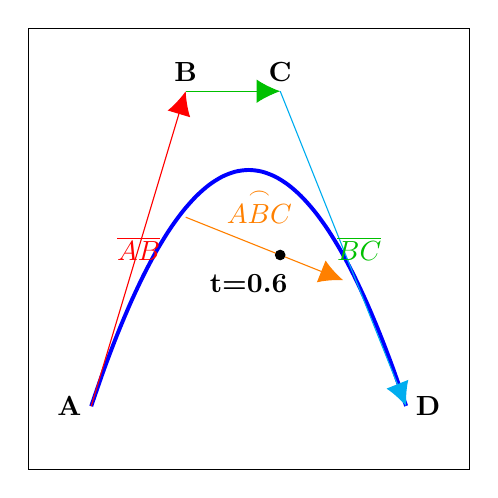
\begin{tikzpicture}[scale=4]
		% border
		\draw (-0.2,-0.2) -- (1.2,-0.2) -- (1.2,1.2) -- (-0.2,1.2) -- (-0.2,-0.2);
		% 1d quadratic bezier curve with control points 0,1,0
		\draw[scale=1,domain=0:1,smooth,variable=\x,blue,line width=0.5mm] plot ({\x},{3*(1-\x)^2*\x+3*\x^2*(1-\x)});		
		% control polygon / labels
		\draw[red,->]       (0.0,0.0) -- (0.3,1.0);
		\draw[darkgreen,->] (0.3,1.0) -- (0.6,1.0);
		\draw[cyan,->]      (0.6,1.0) -- (1.0,0.0);

		\draw[red]          (0.25,0.5) node[anchor=east] {$\overline{AB}$};
		\draw[darkgreen]    (0.75,0.5) node[anchor=west] {$\overline{BC}$};
		% control point labels
		\draw (0.0,0.0) node[anchor=east]  {\bf{A}};
		\draw (0.3,1.0) node[anchor=south] {\bf{B}};
		\draw (0.6,1.0) node[anchor=south] {\bf{C}};
		\draw (1.0,0.0) node[anchor=west]  {\bf{D}};
		% draw a line from AB->AC for time = 0.75
		\draw[orange,->] (0.3,0.6) -- (0.8,0.4);
		\draw[orange] (0.40,0.55) node[anchor=south west] {$\stackrel{\frown}{ABC}$};
		% draw the point at t=0.6 and label underneath the curve
		\draw[black,fill=black] (0.6,0.48) circle (0.015);
		\draw[black] (0.5,0.45) node[anchor=north] {\bf{t}=0.6};
	\end{tikzpicture}
\end{document}